\subsection*{Kinetic Models}
    \begin{definition}[Kinetic model]
        Here, ``kinetic'' models refer to those wherein the distribution of particles positions and velocities is modelled through a single distribution function, as a function of both position and velocity.
    \end{definition}
    For each phase, $s$, we define the (1-particle) distribution function $(f_{s}(\bfx, \bfv; \bft))_{s}$
    \begin{equation}
        f_{s}(\bfx, \bfv; \bft)  :=  \sum_{i}\delta^{3}(\bfx - \bfx_{si})\delta^{3}(\bfv - \bfv_{si})
    \end{equation}
    While working with such $(f_{s})_{s}$ could \emph{in theory} be used to model all the particles exactly and simultaneously, variations of each $f_{s}$ in $\bfx$ occur on the length scale of the distances between particles, i.e. on the order of $10^{- 6}\rmm$ in a tokamak plasma. We would therefore need a mesh resolution on a similar (if not finer) length scale to capture the physical nature of each $f_{s}$. Again: computationally infeasible.

    Since, however, the \emph{precise} position of each particle is generally irrelevant to the general fluid behavior when not working on the atomic scale (in particular on tokamak plasma scales) the key idea of kinetic theory is to model this distribution function as a \emph{random} distribution, as one might do in Bayesian statistics to model a parameter that is known to be of fixed value as a random variable when full information on it is unknown. One defines the 1-particle distribution functions, denoted here as $\left(\widetilde{f}_{s}(\bfx, \bfv)\right)_{s}$, such that $\forall \phi(\bfx, \bfv)$
    \begin{equation}
        \bbE\left\{\int_{\bfx, \bfv}f_{s}(\bfx, \bfv)\phi(\bfx, \bfv)\right\}
        \left(=  \sum_{i}\bbE\{\phi(\bfx_{si}, \bfv_{si})\}\right)
        =  \int_{\bfx, \bfv}\widetilde{f}_{s}(\bfx, \bfv)\phi(\bfx, \bfv)
    \end{equation}
    Similarly the electromagnetic field must be modeled as a random distribution, with $\widetilde{\bfE}$, $\widetilde{\bfB}$ defined, such that $\forall \bfphi(\bfx)$
    \begin{align}
        \bbE\left\{\int_{\bfx}\bfE(\bfx)\cdot\bfphi(\bfx)\right\}  =  \int_{\bfx}\widetilde{\bfE}(\bfx)\cdot\bfphi(\bfx),  && 
        \bbE\left\{\int_{\bfx}\bfB(\bfx)\cdot\bfphi(\bfx)\right\}  =  \int_{\bfx}\widetilde{\bfB}(\bfx)\cdot\bfphi(\bfx)
    \end{align}
    We seek a model in $\left(\widetilde{f}_{s}\right)_{s}$, $\widetilde{\bfE}$, $\widetilde{\bfB}$ \emph{only}.

    \BA{I think I wanna put the precise derivation of the Boltzmann equations in an appendix.}

    To cast an equation from the exact determinstic form to one in these random distribution parameters, one can follow the workflow in Figure \ref{kinetic model construction workflow}.
    \begin{figure}[!h]
        \centering
        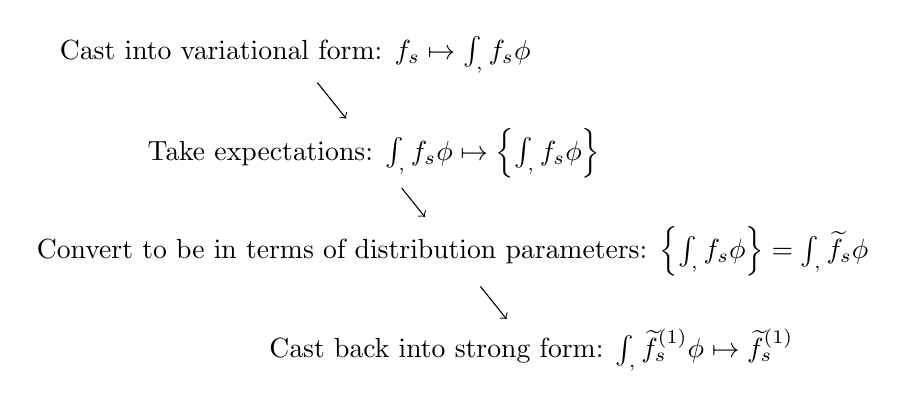
\begin{tikzpicture}[align = center, auto]
            \node (1) at (0, 0) {Cast into variational form: $f_{s}  \mapsto  \int_{\bfx, \bfv}f_{s}\phi$};
            \node (2) at (1, -1.25) {Take expectations: $\int_{\bfx, \bfv}f_{s}\phi  \mapsto  \bbE\left\{\int_{\bfx, \bfv}f_{s}\phi\right\}$};
            \node (3) at (2, -2.5) {Convert to be in terms of distribution parameters: $\bbE\left\{\int_{\bfx, \bfv}f_{s}\phi\right\}  =  \int_{\bfx, \bfv}\widetilde{f}_{s}\phi$};
            \node (4) at (3, -3.75) {Cast back into strong form: $\int_{\bfx, \bfv}\widetilde{f}_{s}^{(1)}\phi  \mapsto  \widetilde{f}_{s}^{(1)}$};

            \draw[->] (1) -- (2);
            \draw[->] (2) -- (3);
            \draw[->] (3) -- (4);
        \end{tikzpicture}
        \caption{Diagram of workflow for contruction of a kinetic model}
        \label{kinetic model construction workflow}
    \end{figure}

    Since this is entirely linear, Maxwell's equations—themselves linear—carry over identically:
    \begin{align*}
        \partial_{t}\widetilde{\bfE}  &=  c^{2}\nabla\wedge\widetilde{\bfB} - \frac{1}{\varepsilon_{0}}\sum_{s}q_{s}\int_{\bfv}\widetilde{f}_{s}\bfv,  &
        \partial_{t}\widetilde{\bfB}  &=  - \nabla\wedge\widetilde{\bfE}  \\
        \nabla\cdot\widetilde{\bfE}  &=  \frac{1}{\varepsilon_{0}}\sum_{s}q_{s}\int_{\bfv}\widetilde{f}_{s},  &
        \nabla\cdot\widetilde{\bfB}  &=  0
    \end{align*}
    As for the evoluation equations for $(f_{s})_{s}$ however, this is sadly \emph{not} the case, due to the non-linear forcing term. \BA{Introduce the 2-particle correlation functions!}

    \BA{Old text...}

    From equations (\ref{patricle motion}–\ref{particle forcing}), we see $(f_{s})_{s}$ satisfy the PDE
    \begin{equation}
        \partial_{t}f_{s} + \nabla_{\bfx}\cdot[f_{s}\bfv] + \frac{q_{s}}{m_{s}}\nabla_{\bfv}\cdot[f_{s}(\bfE + \bfv\wedge\bfB)]  =  0
    \end{equation}
    When considered in isolation, this is referred to as the ``Vlasov'' equation, and can be interpreted as a collision-less version of the Boltzmann equation (\BA{...}).

    \BA{Note here about dropping the tildes from here on out.}
    